% Generated by make_figure.py - do not edit by hand.
\begin{figure}[!ht]
\centering
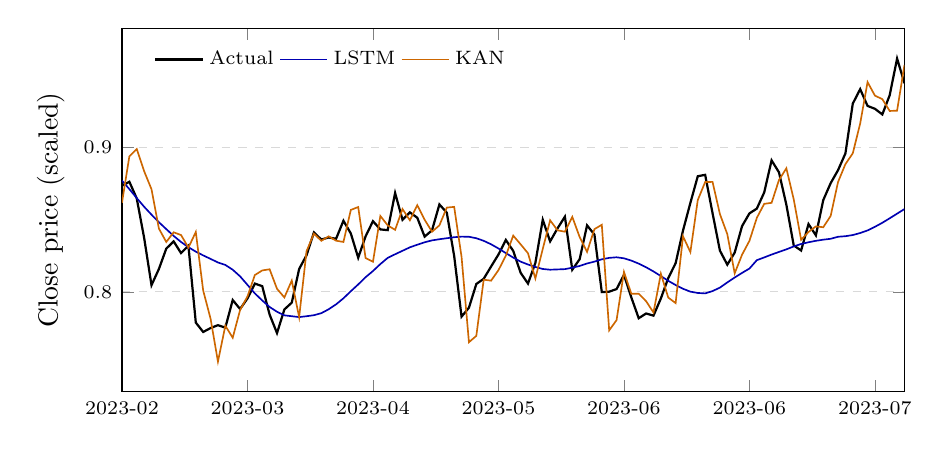
\begin{tikzpicture}
\begin{axis}[
  width=0.95\textwidth, height=6.2cm,
  xmin=0, xmax=106, ylabel={Close price (scaled)},
  xtick={0,17,34,51,68,85,102},
  xticklabels={2023-02,2023-03,2023-04,2023-05,2023-06,2023-06,2023-07},
  x tick label style={font=\scriptsize},
  y tick label style={font=\scriptsize},
  legend style={font=\scriptsize, draw=none}, legend pos=north west,
  legend columns=3, ymajorgrids, grid style={dashed,gray!30}]
\addplot+[mark=none, thick, black] coordinates {
(0,0.8734) (1,0.8762) (2,0.8646) (3,0.8374) (4,0.8046) (5,0.8158) (6,0.8299) (7,0.8349) (8,0.8268) (9,0.8319) (10,0.7787) (11,0.7722) (12,0.7749) (13,0.7769) (14,0.7752) (15,0.7943) (16,0.7881) (17,0.7954) (18,0.8057) (19,0.8039) (20,0.7842) (21,0.7714) (22,0.7878) (23,0.7925) (24,0.8158) (25,0.8253) (26,0.8411) (27,0.8362) (28,0.8376) (29,0.8367) (30,0.8492) (31,0.8404) (32,0.8236) (33,0.8384) (34,0.8489) (35,0.8432) (36,0.8427) (37,0.8684) (38,0.8499) (39,0.8550) (40,0.8513) (41,0.8382) (42,0.8426) (43,0.8605) (44,0.8548) (45,0.8248) (46,0.7828) (47,0.7890) (48,0.8054) (49,0.8090) (50,0.8175) (51,0.8258) (52,0.8359) (53,0.8283) (54,0.8132) (55,0.8057) (56,0.8200) (57,0.8499) (58,0.8349) (59,0.8439) (60,0.8520) (61,0.8153) (62,0.8226) (63,0.8460) (64,0.8396) (65,0.7998) (66,0.8001) (67,0.8019) (68,0.8117) (69,0.7961) (70,0.7817) (71,0.7850) (72,0.7835) (73,0.7954) (74,0.8095) (75,0.8198) (76,0.8424) (77,0.8616) (78,0.8800) (79,0.8810) (80,0.8545) (81,0.8285) (82,0.8188) (83,0.8271) (84,0.8455) (85,0.8543) (86,0.8576) (87,0.8688) (88,0.8910) (89,0.8827) (90,0.8603) (91,0.8321) (92,0.8286) (93,0.8469) (94,0.8391) (95,0.8635) (96,0.8752) (97,0.8842) (98,0.8958) (99,0.9303) (100,0.9403) (101,0.9287) (102,0.9267) (103,0.9228) (104,0.9361) (105,0.9615) (106,0.9444)};
\addplot+[mark=none, semithick, blue!70!black] coordinates {
(0,0.8770) (1,0.8711) (2,0.8649) (3,0.8589) (4,0.8534) (5,0.8482) (6,0.8434) (7,0.8387) (8,0.8345) (9,0.8309) (10,0.8278) (11,0.8252) (12,0.8228) (13,0.8203) (14,0.8186) (15,0.8153) (16,0.8107) (17,0.8048) (18,0.7989) (19,0.7940) (20,0.7895) (21,0.7862) (22,0.7837) (23,0.7831) (24,0.7825) (25,0.7831) (26,0.7838) (27,0.7852) (28,0.7879) (29,0.7913) (30,0.7955) (31,0.8004) (32,0.8051) (33,0.8101) (34,0.8144) (35,0.8192) (36,0.8235) (37,0.8260) (38,0.8284) (39,0.8308) (40,0.8326) (41,0.8343) (42,0.8356) (43,0.8364) (44,0.8371) (45,0.8378) (46,0.8382) (47,0.8381) (48,0.8371) (49,0.8353) (50,0.8329) (51,0.8300) (52,0.8268) (53,0.8237) (54,0.8209) (55,0.8189) (56,0.8172) (57,0.8158) (58,0.8153) (59,0.8155) (60,0.8157) (61,0.8167) (62,0.8179) (63,0.8196) (64,0.8209) (65,0.8225) (66,0.8235) (67,0.8239) (68,0.8232) (69,0.8216) (70,0.8195) (71,0.8170) (72,0.8141) (73,0.8109) (74,0.8076) (75,0.8047) (76,0.8021) (77,0.8001) (78,0.7992) (79,0.7989) (80,0.8005) (81,0.8029) (82,0.8065) (83,0.8099) (84,0.8131) (85,0.8161) (86,0.8219) (87,0.8238) (88,0.8258) (89,0.8276) (90,0.8294) (91,0.8314) (92,0.8331) (93,0.8343) (94,0.8353) (95,0.8361) (96,0.8367) (97,0.8381) (98,0.8385) (99,0.8393) (100,0.8407) (101,0.8425) (102,0.8450) (103,0.8478) (104,0.8509) (105,0.8541) (106,0.8573)};
\addplot+[mark=none, semithick, orange!80!black] coordinates {
(0,0.8617) (1,0.8938) (2,0.8988) (3,0.8835) (4,0.8710) (5,0.8438) (6,0.8345) (7,0.8412) (8,0.8393) (9,0.8306) (10,0.8414) (11,0.8009) (12,0.7814) (13,0.7517) (14,0.7765) (15,0.7682) (16,0.7874) (17,0.7968) (18,0.8116) (19,0.8148) (20,0.8156) (21,0.8021) (22,0.7961) (23,0.8078) (24,0.7824) (25,0.8281) (26,0.8403) (27,0.8353) (28,0.8384) (29,0.8354) (30,0.8345) (31,0.8567) (32,0.8587) (33,0.8234) (34,0.8208) (35,0.8525) (36,0.8460) (37,0.8429) (38,0.8573) (39,0.8495) (40,0.8600) (41,0.8499) (42,0.8416) (43,0.8460) (44,0.8583) (45,0.8588) (46,0.8242) (47,0.7651) (48,0.7695) (49,0.8084) (50,0.8077) (51,0.8150) (52,0.8250) (53,0.8389) (54,0.8329) (55,0.8267) (56,0.8092) (57,0.8297) (58,0.8495) (59,0.8426) (60,0.8416) (61,0.8519) (62,0.8379) (63,0.8276) (64,0.8434) (65,0.8464) (66,0.7733) (67,0.7804) (68,0.8138) (69,0.7986) (70,0.7987) (71,0.7935) (72,0.7857) (73,0.8125) (74,0.7960) (75,0.7922) (76,0.8384) (77,0.8275) (78,0.8635) (79,0.8760) (80,0.8761) (81,0.8538) (82,0.8399) (83,0.8128) (84,0.8257) (85,0.8353) (86,0.8512) (87,0.8609) (88,0.8616) (89,0.8774) (90,0.8855) (91,0.8640) (92,0.8360) (93,0.8414) (94,0.8453) (95,0.8447) (96,0.8525) (97,0.8760) (98,0.8884) (99,0.8959) (100,0.9165) (101,0.9452) (102,0.9358) (103,0.9334) (104,0.9252) (105,0.9254) (106,0.9570)};
\legend{Actual, LSTM, KAN}
\end{axis}
\end{tikzpicture}
\caption{TODO write caption}
\label{fig:figure_h2_step1_s0_pykan}
\end{figure}
